% \subsection{Program-Based Data Dependency Graph Generation}
% %  Weighted Data Dependency Graph Generation}
%  \label{sec:alg_graphgen}
 %
%    Each directed edge represents an abstract transition 
%    between two control locations, i.e., the labels of two commands (we call the labels also control location and they refer to the same thing in the follows), 
%    where the second labeled command will be executed after execution of the command with first label.
%    The abstract transition contains a set of difference constraints for variables, generated by abstracting the command of the first label.
%   \item Computing 
%   % I get the reachability bound for each command.
%   the symbolic reachability bound for each command,
%   % the value bound invariant for each variable in the event and 
%   by inferring the value bound invariant for each variable 
%   % the event transition closure over the abstract control flow graph,
%   and the transition closure for every abstract transition through the constraints over the abstract control flow graph.
%   % \\
%   % Through this graph and constraint for every transition, I infer the  invariant for every variable,
%   % and compute the transition closure for every abstract transition.
%   % By solving the closure with the invariants of variables involved in this closure for every transition, 
%   % I compute the symbolic reachability bound of every commands corresponding to 
% %     % this transition.
% %     \item Performing a feasible data-flow analysis from the reachable definition algorithm. 
% % %  By generating set of all the reachable variables at location of label $l$ in the program $c$.
% % and generating the set of all the reachable variables for every program location.
% % For every labelled variable $x^l$ in this set, 
% % the value assigned to that variable
% % in the assignment command associated to that label is reachable at the entry point of  executing the command of label $l$.
% % \item Refining the abstract control flow graph into a weighted-data dependency graph, 
% % by annotating each vertex with reachability bounds and 
% % removing unfeasible edges and redundant edges and vertices.
% % adding edges between
% %     variables having data-flow relations, and
% % removing the edges between locations where the variables associated to that labeled command isn't reachable from the second location.
% % \\
% % first annotate each vertex of label $l$ with the variable 
% % assigned in that labeled command, and remove the rest doesn't correspond to an assignment command.
% % Then 
% % add direct edge between two labeled variables,
% % where the first variable 
% % is directly used in the assignment expression to the second variable, by restricting 
% % the first labeled variable is reachable at the the second label.
% %
% \item Computing the adaptivity through this weighted data dependency graph,
%   by finding a finite walk on this weighted graph, 
% traversing the maximum times of query variables, by restricting the visiting time of every vertex on this walk to its weight.
% The maximum number of vertices corresponding to a query variables visited on this walk is the estimated upper bound, for program's adaptivity.

%    In this step, $\THESYSTEM$ refines the abstract control flow graph into the program-based weighted-data dependency graph, 
% by annotating each vertex with reachability bounds and 
% removing unfeasible edges and redundant edges and vertices,
% % This graph is used 
% for approximating the trace-based weight-data dependency graph.
% \\
% Specifically, I first annotate each vertex of label $l$ with the variable 
% assigned in that labeled command, and remove the rest doesn't correspond to an assignment command.
% Then 
% add direct edge between two labeled variables,
% where the first variable 
% is directly used in the assignment expression to the second variable, by restricting 
% the first labeled variable is reachable at the second label.
% % \\
% The formal definition is as follows.
Based on the variable \emph{may-dependency} relation in Section~\ref{sec:dynamic-datadep} and 
the dependency quantity analysis in Section~\ref{sec:dynamic-reachability}.
% gives us the edges, 
I firstly define the execution-based dependency graph, then formalize the \emph{adaptivity} in this section.

\subsubsection{Program-Based Data Dependency Graph Generation}
%  Weighted Data Dependency Graph Generation}
 \label{sec:alg_graphgen}
 To build the graph, we firstly estimate the vertices and query annotations straightforwardly as follows.
\paragraph{Vertices Estimation and Query Annotation Estimation}
\label{sec:alg_vertexgen}
The vertices in the static analysis dependency graph are actually identical as the  Execution-Based Dependency Graph, which are assigned variables in the program annotated with the unique label(line number). These vertices are collected by statically scanning the program, like what I do for vertices of its Execution-Based Dependency Graph. The vertices are defined formally as follows.

  \highlight{
\[
    \progV(c) \triangleq \left\{ 
  x^l \in \mathcal{LV} 
  ~ \middle\vert ~
  x^l \in \lvar_{c}
  \right\}
  \]
  }
  %

The static scanning of the programs also tells us whether one vertice(assigned variable) is assigned by a query request.  I have similar definition when defining the Execution-Based Dependency Graph, 
a set of pairs $\progF(c) \in \mathcal{P}(\mathcal{LV} \times \{0, 1\} )$ 
% is the set of pairs 
% The weight for each vertex in $\progV(c)$ is computed 
mapping each $x^l \in \progV(c)$ to a flag, either $0$ or $1$, where $1$  means $x^{l}$ is a member of $ \qvar_{c}$, a set of those variables assigned with query requests, and $0$ means $x^{l}$ not in this set. It is defined formally below.

\[\progF(c) =\left\{(x^l, n)  \in  \mathcal{LV} \times \{0, 1\} 
~ \middle\vert ~
x^l \in \lvar_{c},
n = 1 \iff x^l \in \qvar_{c} \land n = 0 \iff  x^l \not\in \qvar_{c} .
\right\}\]

Then, I build the estimated data dependency graph based on the above program static analysis as follows:
\\
\highlight{
\[
  \progG(c) = (\progV(c), \progE(c), \progW(c), \progF(c))
  \]
}
with $\progV(c), \progE(c), \progW(c)$ and $ \progF(c)$ as computed in each steps above.
% and $\progF(c) =\left\{(x^l, n)  \in  \mathcal{LV} \times \{0, 1\} 
% ~ \middle\vert ~
% x^l \in \lvar_{c},
% n = 1 \iff x^l \in \qvar_{c} \land n = 0 \iff  x^l \in \qvar_{c} .
% \right\} $,
This program-based graph program-based graph has a similar topology structure as 
% the one
% of 
the Execution-Based Dependency Graph. It has the same
vertices and query annotations, but approximated edges and weights.  
% The algorithm computation is 
It is formally defined in Definition~\ref{def:prog_graph}.
% Through the reachable definition set on every label,
% I remove the edges between labels where the variables associated to that labeled command isn't reachable from the second location.
%\absG(c) =(\absV, \absE, \absW)
\begin{defn}
[Program-Based Dependency Graph]
\label{def:prog_graph}
% [Program-Based Weighted Data Dependency Graph Generation Algorithm]
% \label{def:analyz_dcfg}
Given a program $c$, with its abstract weighted control flow graph $\absG(c) = (\absV, \absE, \absW)$ and 
feasible data flow relation $\flowsto(x^i, y^j, c)$ for every $x^i, y^j \in \lvar_c$, its Program-Based Weighted Data Dependency Graph
$\progG(c) = (\progV, \progE, \progW, \progF)$,
is generated as follows,
% \\
% \highlight{
% $\progV =\{x^l | x^l \in \lvar_c\} $
% \\
% $\progE = \{(y^i, x^l) | (y^i, x^l)  \in dcdg(c) \}$
% \\
% $\progW = \{(x^l, w ) | (l, w ) \in \absW \land x^l \in \lvar_c\}$
% \\
% $\progF = \{(l, q) \in \mathcal{L} \times \{0, 1\}| q = 1 \iff l \in \qvar_c, q = 0 \iff l \notin \qvar_c \}$.
% }
% \end{defn}
% \begin{defn}
% [Program-Based Dependency Graph].
% \label{def:prog_graph}
%   % \\
% Given a program ${c}$
% its program-based graph 
% $\progG({c}) = (\vertxs, \edges, \weights, \qflag)$ is defined as:
{\footnotesize
\[
\begin{array}{rlcl}
\text{Vertices} &
\progV & := & \left\{ 
x^l \in \mathcal{LV} 
~ \middle\vert ~
x^l \in \lvar_{c}
\right\}
\\
\text{Directed Edges} &
\progE & := & 
\left\{ 
({x}_1^{i}, {x}_2^{j}) \in \mathcal{LV} \times \mathcal{LV}
~ \middle\vert ~
\begin{array}{l}
{x}_1^{i}, {x}_2^{j} \in \vertxs
\land
% \\
\exists n \in \mathbb{N}, z_1^{r_1}, \cdots, z_n^{r_n} \in \lvar_{{c}} \sthat  
n \geq 0 \land
\\
\flowsto(x^i,  z_1^{r_1}, c) 
\land \cdots \land \flowsto(z_n^{r_n}, y^j, c) 
\end{array}
\right\}
\\
\text{Weights} &
\progW & := &
% \bigcup
% \begin{array}{l}
\left\{ (x^l, w) \in  \mathcal{LV} \times \mathcal{A}_{in}
\mid
x^l \in \lvar_{{c}} \land (l, w) \in \absW(c)
\right\}
% \end{array} 
\\
\text{Query Annotation} &
\progF & := & 
\left\{(x^l, n)  \in  \mathcal{LV} \times \{0, 1\} 
~ \middle\vert ~
x^l \in \lvar_{c},
n = 1 \iff x^l \in \qvar_{c} \land n = 0 \iff  x^l \in \qvar_{c} .
\right\}
\end{array}
\] }
\end{defn}

Then, the Following part computes the adaptivity upper bound for a program $c$.
% Given a program ${c}$, we generate
\\
With
% its 
$c$'s program-based data dependency graph $\progG({c})$ approximated above,
%
its adaptivity upper bound 
% Defined in Definition~\ref{def:prog_adapt} as 
%
is estimated as
the maximum query length over all finite walks in $\walks(\progG({c}))$ formally in Definition~\ref{def:prog_adapt}, 
and computed 
% is computed as the maximum query length over all finite walks in $\walks(\progG({c}))$, and computed 
in Algorithm~\ref{alg:adpt_alg}.
% We use $\walks(\progG(c))$ represents the walks over the program-based dependency graph for $c$.
Different from the finite walk on a program $c$'s execution based graph,
%  $\traceG(c)$, 
% $k \in \walks(\progG(c))$ 
the finite walk in $\progG(c)$ doesn't rely on initial trace.
The occurrence times of every $v_i $ in $k$'s vertex sequence is bound by 
an arithmetic expression $w_i$ where $(v_i, w_i) \in \progW(c)$, is $v_i$'s estimated weight. 
% Then $\qlen(k) \in \mathcal{A}_{in}$ as well. 
% The full definition for $\walks(\progG(c))$ and $\qlen$ over $\walks(\progG(c))$ is in Apdix.
%
Formally defined as follows.
\begin{defn}[Finite Walk on Program-Based Dependency Graph ($k$)]
  \label{def:prog_finitewalk}
  Given a program $c$'s program-based dependency graph 
  $\progG({c}) = (\progV(c), \progE(c), \progW(c), \progF(c))$, 
  a \emph{finite walk} $k$ in $\traceG({c})$ is
  % function $k: \mathcal{T} \to $ 
  % sequence of edges.
  % For a initial trace $\trace_0 \in \mathcal{T}$, 
  % $k(\trace_0)$ is
  a sequence of edges $(e_1 \ldots e_{n - 1})$ 
  for which there is a sequence of vertices 
  $(v_1, \ldots, v_{n})$ such that:
  \begin{itemize}
      \item $e_i = (v_{i},v_{i + 1}) \in \progE(c)$ for every $1 \leq i < n$.
      \item every vertex $v_i \in \progV(c)$,
      and $(v_i, w_i) \in \progW(c)$, 
       $v_i$ appears in $(v_1, \ldots, v_{n})$ at most 
    $w_i$
      times.  
  \end{itemize}
  %
  The length of $k$ is the number of vertices in its vertex sequence, i.e., $\len(k) = a$.
 \end{defn}
  We abuse the notation $\walks(\progG(c))$ represents the walks over the program-based dependency graph for $c$.
Different from the walks on a program $c$'s execution based graph,
 $k \in \walks(\traceG(c))$, 
$k \in \walks(\progG(c))$ doesn't rely on initial trace.
The occurrence times of every $v_i $ in $k$'s vertex sequence is bound by 
an arithmetic expression $w_i$ where $(v_i, w_i) \in \progW(c)$, is $v_i$'s estimated weight. 
% Notice here, for a walk in $\progG(c)$, the occurrence times of every vertex in vertices sequence, 
%  and its 
 The length of a finite walk $k \in \walks(\progG(c))$ is an arithmetic expression
 as well, i.e., $\len(k) \in \mathcal{A}_{in}$

 Then the query length of a finite walk in  $\progG(c)$ is an arithmetic expression as well as follows,
%  $\qlen(k) \in \mathcal{A}_{in}$ as well. 
% The adaptivity upper bound 
% is estimated as
% Then the adaptivity bound based on program analysis for ${c}$ 
% is the number of query vertices on a finite walk in $\progG({c})$. This finite walk satisfies:
% \begin{itemize}
% \item the number of query vertices on this walk is maximum
% \item the visiting times of each vertex $v$ on this walk is bound by its reachability bound $\weights(v)$.
% \end{itemize}
\begin{defn}[Query Length of the Finite Walk on Program-Based Dependency Graph ($\qlen$)]
  \label{def:static-qlen}
  Given 
  % labelled weighted graph $G = (\vertxs, \edges, \weights, \qflag)$, 
  a program $c$'s execution-based dependency graph 
  $\progG({c}) = (\progV(c), \progE(c), \progW(c), \progF(c))$, 
   and a \emph{finite walk} $k \in \walks(\progG(c))$,
  The query length of $k$, $\qlen(k) \in \mathcal{A}_{in}$ 
  % is a function $\qlen(k): \mathcal{T} \to \mathbb{N}$, such that with an initial trace  $\trace_0 \in \mathcal{T}$, 
  % $\qlen(k)(\trace_0)$ 
  is the number of vertices which correspond to query variables in the vertices sequence of this walk $k$
  $(v_1, \ldots, v_{n})$ as follows, 
  \[
    \qlen(k) = |\big( v \mid v \in (v_1, \ldots, v_{n}) \land \qflag(v) = 1 \big)|.
  \]
  % , where $\trace_0 \in \mathcal{T}$ is the initial trace and $\big(v \mid v \in (v_1, \ldots, v_{n}) \land \qflag(v) = 1 \big)$ is a subsequence of $(v_1, \ldots, v_{n})$.
  %  $k$'s vertex sequence.
  % \mg{If I understand where you want to go, why don't you just use the cardinality of the set above, rather than taking the length of a subsequence?}
  % \jl{because the same vertex could have multiple occurrence in the sequence, and we will count all the occurrence instead of just once.
  % So the cardinality of set doesn't work.}
  \end{defn}
% is computed as the maximum query length over all finite walks in $\walks(\progG({c}))$, and computed 
% It is formally defined in \ref{def:prog_adapt}.
% defined formally as follows.
%
\subsubsection{Program-Based Adaptivity Computation}
%  Weighted Data Dependency Graph Generation}
 \label{sec:static-adapt-comput}
%
\begin{defn}
[{Program-Based Adaptivity}].
\label{def:prog_adapt}
\\
{
Given a program ${c}$ and its program-based graph 
$\progG({c})$
%  = (\vertxs, \edges, \weights, \qflag)$,
%
the program-based adaptivity for $c$ is 
% a function $\progA({c}): \mathcal{T} \to\mathbb{N} $,
% for an initial trace $\trace_0 \in \mathcal{T}$,
defined as%
\[
\progA({c})
\triangleq \max
\left\{ \qlen(k) \ \mid \  k \in \walks(\progG(c))\right \}.
\]
}
\end{defn}
Based on our soundness of the program-based adaptivity, our program-based adaptivity is a sound upper bound of its adaptivity in Definition~\ref{def:trace_adapt}. 
\begin{thm}[Soundness of \THESYSTEM]
    \label{thm:sound_progadapt}
    For every program $c$, 
    % for any initial trace $\trace_0$, 
    its program-based adaptivity is a sound upper bound of its adaptivity.
     $$  \progA(c) \geq A(c)$$
\end{thm}
For $\progA(c) \geq A(c)$ comparing between function and arithmetic expression,
we are specifically comparing, $\forall \trace \in \mathcal{T} \sthat  
\config{A(c), \trace} \earrow n \implies n \geq A(c)(\trace) $.
To estimate a sound and precise upper bound on adaptivity, we develop an adaptivity estimation algorithm called $\pathsearch$ (in Apdix Algorithm~I), which uses both the deep first search and breath first search strategy to find the walk. We also show that the estimated adaptivity from our $\pathsearch$ is sound with respect to the program-based adaptivity. 
\begin{thm}[Soundness of $\pathsearch$]
    \label{thm:sound_adaptalg}
    For every program $c$.
    % for any initial trace $\trace_0$,
     $$\pathsearch(\progG({c})) \geq \progA(c).$$
\end{thm}
The full details of all the soundness can be found in the appendix.
% The following algorithm finds the walk with the longest query length on a program $c$'s execution-based dependency graph 
% $\progG(c)$
% %  = (\vertxs, \edges, \weights, \qflag)$, 
% through a combination of 
% % DFS and BFS algorithm 
% deep first search and breath first search strategy
% % as defined 
% in Algorithm~\ref{alg:adpt_alg} and Algorithm~\ref{alg:adaptscc}.

% \paragraph*{Challenges}
% Following is the challenge of computing the adaptivity on a program based dependency graph.
% \\
% In order to 
% % search for the finite walk having the longest query length, which isn't a simple longest weighted path.
% compute the adaptivity for a program $c$ on its estimated Program-Based Dependency Graph $\progG(c)$, we need to 
% search for the finite walk having the longest query length.
% \\
% % However, the finite walk isn't a simple weighted path by Definition~\ref{def:finitewalk}, there are two challenges in order to find this walk.
% However, by Definition~\ref{def:finitewalk}, this finite walk isn't easy to find, below are the challenges in order to find this walk.
% \\
% \textbf{Non-Termination Challenge:}
% % Moreover, b
% We can neither simply traverse on this graph by decreasing the weight of every node by one after every visiting. 
% The simple 
% traversing strategy leads to non-termination for most programs. 
% Specifically, this challenge comes from the weight of each vertex estimated in program's Program-Based Dependency Graph,
% which isn't a number but a symbolic expression. 
% % because the weight is symbolic and simply traversing leads to non-termination.
% It is difficult to tell when to terminate the recursion when the domain of this symbolic expression isn't finite,
% while, in most of our cases, the programs' Program-Based Dependency Graphs are having symbolic weights with infinite domains on vertices.
% \todo{for example:}
% Look at the simple example in Figure~\ref{fig:alg_adaptsearch_simplewhile}, where $k$ is the input variable from domain $\mathbb{N}$,
% %  in Figure~\ref{} in Section~\ref{sec:overview},
% \begin{figure}
% \centering
% {\footnotesize
% \begin{subfigure}{.25\textwidth}
% \begin{centering}
% $ 
% \begin{array}{l}
%   \kw{whileSim(k)} \triangleq \\
%   \clabel{ \assign{j}{k} }^{0} ; \\
%   \clabel{ \assign{x}{\query(\chi[0])} }^{1} ; \\
%       \ewhile ~ \clabel{j > 0}^{2} ~ \edo ~ \\
%       \Big(
%        \clabel{\assign{x}{\query(\chi[x]) }}^{3}  ; \\
%       \clabel{\assign{j}{j-1}}^{4}       \Big)
%   \end{array}
% $
% \caption{}
% \end{centering}
% \end{subfigure}
% \quad
%   \begin{subfigure}{.6\textwidth}
%   \begin{centering}
%   \begin{tikzpicture}[scale=\textwidth/18cm,samples=200]
% \draw[] (0, 7) circle (0pt) node
% {\textbf{$x^1: {}^{1}_{1}$}};
% \draw[] (0, 4) circle (0pt) node
% {{ $x^3: {}^{k}_{1}$}};
% % Counter Variables
% \draw[] (5, 9) circle (0pt) node {{$j^2: {}^{1}_{0}$}};
% \draw[] (5, 6) circle (0pt) node {{ $j^4: {}^{k}_{0}$}};
% %
% % Value Dependency Edges:
% \draw[ ultra thick, -latex, densely dotted,] (0, 4.5)  -- (0, 6.5) ;
% \draw[ ultra thick, -latex, densely dotted,] (0.5, 4.2) arc (150:-180:1);
% \draw[ thick, -Straight Barb] (5.5, 6.2) arc (150:-150:1);
% \draw[ thick, -latex] (5, 6.5)  -- (5, 8.5) ;
% % Control Dependency
% \draw[ thick,-latex] (1.5, 7)  -- (4, 9) ;
% \draw[ thick,-latex] (1.5, 4)  -- (4, 9) ;
% \draw[ thick,-latex] (1.5, 7)  -- (4, 6) ;
% \draw[ thick,-latex] (1.5, 4)  -- (4, 6) ;
% \end{tikzpicture}
% \caption{}
%   \end{centering}
%   \end{subfigure}
% }
% % \end{wrapfigure}
% % \end{equation*}
% \vspace{-0.4cm}
%  \caption{(a) Simple While Loop Example, (b) Execution-Based Dependency Graph, (c) The Static Program-Based Dependency graph.}
% \label{fig:alg_adaptsearch_simplewhile}
% \vspace{-0.5cm}
% \end{figure}
% % Analysis Results: $ \progA(\kw{whileRec}(k)) = 1 + k$
% %
% If we traverse on it's $\progG(c)$, and decrease the weight of $x^3$ by one after every visit,
% % We can simply adopt either a deep first strategy to estimate the adaptivity as the length of the longest weight path, as 
% % in Algorithm~\ref{alg:overadp_alg}.
% we will never terminate because we only know $k \in \mathbb{N}$.
% % However, this gives us over-approximation to a large extend.
% % In Algorithm~\ref{alg:adpt_alg}, 
% % we first find all the strong connected components of this graph, 
% \\
% \textbf{Approximation Challenge:}
% % As in Definition~\ref{def:finitewalk}, w
% We cannot 
% % simply adopt either a deep first strategy to estimate the adaptivity as the length of the longest weight path, as in Algorithm~\ref{alg:overadp_alg}.
% simply adopt a deep first strategy to 
% search for the longest weighted path
% estimate the adaptivity as the weighted query length of this path
% % of the longest weight path, 
% as in Algorithm~\ref{alg:overadp_alg}.
% % However, this gives us over-approximation to a large extend.
% It is easy to see that this gives us over-approximation to a large extend.
% \\
% Specifically, according to the finite walk definition in Definition~\ref{def:finitewalk},
% the visiting time of every vertex on a walk should be no more than its weight.
% % which is a symbolic expression.
% % So we cannot simply 
% However, by searching for the longest weighted path, 
% % and approximating the finite walk by this weight path, 
% and use it as the approximated finite walk with the longest query length, 
% the visiting times of the vertex on 
% % it 
% this approximated walk could 
% % possibly 
% exceed 
% % its weights. 
% the visiting times it can have.
% Then, this approximated walk isn't a qualified walk by Definition~\ref{def:finitewalk}, 
% and the weighted query length of this path is obviously greater than the maximum query length of the finite walk.
% This over-approximation could result in a $\infty$ adaptivity upper bound on the program with actual adaptivity $2$.
% \todo{For example}
% \\
% Look at the two-round example in overview, 
% it is easy to find that the longest weighted path is  $x^3 : {}^{k}_{1} \to a^5 : {}^{k}_{0} \to l^6 : {}^{1}_{0}$ with weighted query length $1 + k$.
% If we use this path to approximate a finite walk, and weight of each vertex as
% %  their visiting times, 
% its visiting time,
% then it isn't a qualified walk. 
% In the approximated walk, we have the vertices as $x^3 \to \cdots \to x^3 \to a^5 \to \cdots \to a^5 \to l^6$.
% Because $l^6$ can only be visited as most once by its weight,
% % and this lead to 
% resulting in the restriction on the maximum visiting time of $x^3$,
% such that $x^3$ is only able to be visited at most once as well.
% %
% However, $x^3$ is visited $k$ times in this approximated walk.
% % Moever, with the longest query length, then 
% In order to have $x^3$ be visited $k$ time, we need to go back to 
% $x^3$ on this walk from either $a^5$ or $l^6$ for $k$ time.
% This is impossible since there is no edge going back to $x^3$ in $\progG(twoRound)$.
% Obviously,
% % the with the weighted length $1 + k$. It is obviously
% its weighted query length, $1 + k$, 
% % which is 
% over approximates 
% % its 
% the adaptivity of this example to a large extend, which supposed to be $2$. 
% %  for this program, 
% % that 
% \\
As indicated by our definition of prograpm-based adaptivity, the key point is to find the walks in the program-based dependency graph. We develop some walk-finding algorithms,  Algorithm~\ref{alg:adpt_alg} and Algorithm~\ref{alg:adaptscc}, which use both the deep first search and breath first search strategy.  

By Definition~\ref{def:finitewalk}, this finite walk isn't easy to find. We first discuss two challenges when we try to find the walks in the dependency graph, and show that how we solve them using our algorithms.

% \paragraph*{Challenges}
% Following is the challenge of computing the adaptivity on a program based dependency graph.
% \\
% In order to 
% % search for the finite walk having the longest query length, which isn't a simple longest weighted path.
% compute the adaptivity for a program $c$ on its estimated Program-Based Dependency Graph $\progG(c)$, we need to 
% search for the finite walk having the longest query length.
% \\
% % However, the finite walk isn't a simple weighted path by Definition~\ref{def:finitewalk}, there are two challenges in order to find this walk.
% However, by Definition~\ref{def:finitewalk}, this finite walk isn't easy to find, below are the challenges in order to find this walk.
% \\
\textbf{Non-Termination Challenge:}
% Moreover, b
One naive walk finding method is to simply traverse on this graph by decreasing the weight of every node by one after every visiting. However, this simple 
traversing strategy leads to non-termination dilemma for most programs we are interested in. 
Specifically, this challenge comes from the weight of each vertex estimated in program's Program-Based Dependency Graph,
which is not only a number but also can be a symbolic expression. 

% because the weight is symbolic and simply traversing leads to non-termination.
It is difficult to tell when to terminate the recursion when the domain of this symbolic expression isn't finite, some the walk may also be infinite.
While, in most of our cases, the programs' Program-Based Dependency Graphs are having symbolic weights with infinite domains on vertices.
Look at the simple example in Figure~\ref{fig:alg_adaptsearch_simplewhile}, where $k$ is the input variable from domain $\mathbb{N}$.
%  in Figure~\ref{} in Section~\ref{sec:overview},
\begin{figure}
\centering
{
% \footnotesize
\begin{subfigure}{.25\textwidth}
\begin{centering}
$ 
\begin{array}{l}
  \kw{whileSim(k)} \triangleq \\
  \clabel{ \assign{j}{k} }^{0} ; \\
  \clabel{ \assign{x}{\query(\chi[0])} }^{1} ; \\
      \ewhile ~ \clabel{j > 0}^{2} ~ \edo ~ \\
      \Big(
       \clabel{\assign{x}{\query(\chi[x]) }}^{3}  ; \\
      \clabel{\assign{j}{j-1}}^{4}       \Big)
  \end{array}
$
\caption{}
\end{centering}
\end{subfigure}
\quad
  \begin{subfigure}{.6\textwidth}
  \begin{centering}
  \begin{tikzpicture}[scale=\textwidth/18cm,samples=200]
\draw[] (0, 7) circle (0pt) node
{\textbf{$x^1: {}^{1}_{1}$}};
\draw[] (0, 4) circle (0pt) node
{{ $x^3: {}^{k}_{1}$}};
% Counter Variables
\draw[] (5, 9) circle (0pt) node {{$j^2: {}^{1}_{0}$}};
\draw[] (5, 6) circle (0pt) node {{ $j^4: {}^{k}_{0}$}};
%
% Value Dependency Edges:
\draw[ ultra thick, -latex, densely dotted,] (0, 4.5)  -- (0, 6.5) ;
\draw[ ultra thick, -latex, densely dotted,] (0.5, 4.2) arc (150:-180:1);
\draw[ thick, -Straight Barb] (5.5, 6.2) arc (150:-150:1);
\draw[ thick, -latex] (5, 6.5)  -- (5, 8.5) ;
% Control Dependency
\draw[ thick,-latex] (1.5, 7)  -- (4, 9) ;
\draw[ thick,-latex] (1.5, 4)  -- (4, 9) ;
\draw[ thick,-latex] (1.5, 7)  -- (4, 6) ;
\draw[ thick,-latex] (1.5, 4)  -- (4, 6) ;
\end{tikzpicture}
\caption{}
  \end{centering}
  \end{subfigure}
}
% \end{wrapfigure}
% \end{equation*}
\vspace{-0.4cm}
 \caption{(a) Simple While Loop Example, (b) The Program-Based Dependency Graph generated from $\THESYSTEM$.}
\label{fig:alg_adaptsearch_simplewhile}
\vspace{-0.5cm}
\end{figure}
% Analysis Results: $ \progA(\kw{whileRec}(k)) = 1 + k$
%
If we traverse on the program-based dependency graph, and decrease the weight of $x^3$ (the weight $k$ is symbolic) by one after every visit,
% We can simply adopt either a deep first strategy to estimate the adaptivity as the length of the longest weight path, as 
% in Algorithm~\ref{alg:overadp_alg}.
we will never terminate because we only know $k \in \mathbb{N}$.

To solve this non-termination challenge, we switch to another walk finding approach: we first find a  longest path in the program-based dependency graph and then approximate the walk with the path.
Through a simple deep first search algorithm, we find the longest weighted path as the dotted arrow in Figure~\ref{fig:alg_adaptsearch_simplewhile},
$x^3: {}^k_1 \to x^1: {}^1_1 $.
Then, by summing up the weights on this path where the vertices has query annotation $1$, deep first search algorithm gives the adaptivity bound $1 + k$.
This is a the tight bound for this program's adaptivity.
% Look at the two-round example in overview, 
% it is easy to find that the longest weighted path is  $x^3 : {}^{k}_{1} \to a^5 : {}^{k}_{0} \to l^6 : {}^{1}_{0}$ with weighted query length $1 + k$.
% If we use this path to approximate a finite walk, and weight of each vertex as
% %  their visiting times, 
% its visiting time,
% then it isn't a qualified walk. 
% In the approximated walk, we have the vertices as $x^3 \to \cdots \to x^3 \to a^5 \to \cdots \to a^5 \to l^6$.

% However, this gives us over-approximation to a large extend in other cases as in \textbf{Approximation Challenge}.
% In Algorithm~\ref{alg:adpt_alg}, 
% we first find all the strong connected components of this graph, 
\textbf{Approximation Challenge:}
% As in Definition~\ref{def:finitewalk}, w
When we adopt a deep first strategy to search for the longest weighted path, and then use the path to approximate the adaptivity. We find that this gives us over-approximation to a large extend.
% Specifically, according to the finite walk definition in Definition~\ref{def:finitewalk},
% the visiting time of every vertex on a walk should be no more than its weight.
% However, by searching for the longest weighted path, 
% % and approximating the finite walk by this weight path, 
% and use it as the approximated finite walk with the longest query length, 
% the visiting times of the vertex on 
% % it 
% this approximated walk could 
% % possibly 
% exceed 
% % its weights. 
% the visiting times it can have.
% Then, this approximated walk isn't a qualified walk by Definition~\ref{def:finitewalk}, 
% and the weighted query length of this path is obviously greater than the maximum query length of the finite walk.
This over-approximation could result in a $\infty$ adaptivity upper bound on the program with actual adaptivity $2$.
Look at the two-round example in overview, 
it is easy to find that the longest weighted path is  $x^3 : {}^{k}_{1} \to a^5 : {}^{k}_{0} \to l^6 : {}^{1}_{0}$ with weighted query length $1 + k$.
If we use this path to approximate a finite walk, and weight of each vertex as
%  their visiting times, 
its visiting time,
then it isn't a qualified walk. 
In the approximated walk, we have the vertices as $x^3 \to \cdots \to x^3 \to a^5 \to \cdots \to a^5 \to l^6$.
Because $l^6$ can only be visited as most once by its weight,
% and this lead to 
resulting in the restriction on the maximum visiting time of $x^3$,
such that $x^3$ is only able to be visited at most once as well.
%
However, $x^3$ is visited $k$ times in this approximated walk.
% Moever, with the longest query length, then 
In order to have $x^3$ be visited $k$ time, we need to go back to 
$x^3$ on this walk from either $a^5$ or $l^6$ for $k$ time.
This is impossible since there is no edge going back to $x^3$ in $\progG(twoRound)$.
Obviously,
% the with the weighted length $1 + k$. It is obviously
its weighted query length, $1 + k$, 
% which is 
over approximates 
% its 
the adaptivity of this example to a large extend, which supposed to be $2$. 
%  for this program, 
% that 


These challenges motivate us to design a walk search algorithm through a combination of 
% DFS and BFS algorithm 
deep first search and breath first search strategy. 
% \wq{
This walk search algorithm consists of two components:
the path searching algorithm, $\pathsearch$ (in Algorithm~\ref{alg:adpt_alg})
which search for a 'suitable' path relying on the strong connected components of the program based dependency graph, 
and $\kw{\pathsearch_{scc}(G)}$ (in Algorithm~\ref{alg:adaptscc}) which approximates the
path.
% path found by Algorithm~\ref{alg:adpt_alg} 
% to a precise walk on the SCC
% and computes the adaptivity.
% These challenges give us the necessary to design a walk search algorithm through a combination of 
% % DFS and BFS algorithm 
% deep first search and breath first search strategy
% % as defined 
% as in Algorithm~\ref{alg:adpt_alg} and Algorithm~\ref{alg:adaptscc}.
%
The $\pathsearch$ as shown in Appendix Algorithm~I, takes our program-based dependency graph as input, and outputs the estimated adaptivity by two steps. 1. Process the input graph to a simplified graph 2. Perform
     the standard breath first search strategy to find the longest weighted path on this simplified graph and return the length as adaptivity.
The step 2 is not interesting, we now discuss step 1. 
The input dependency graph may contain circle due to the while loop, we simplify (shrank) the input graph by replacing every strong connected components(circle) of the graph with, the vertex whose weight is the adaptivity of the SCC 
(a subgraph of the input one) calculated by the $\pathsearch_{\kw{scc}}$. 
The SCC is found by using the Kosaraju's algorithm.
% \wq{cite}. 
The details of this algorithm is explained as follows.
    % This algorithm first finds all the strong connected components (SCC) of $\progG(c)$ using the Kosaraju’s algorithm in line:3. 
    % Every $\kw{SCC_1}, \cdots, \kw{SCC_n}$
    % where $0 \leq n \leq |\vertxs|$ is a sub-graph of $\progG(c)$, where $\kw{SCC_i} = (\vertxs_i, \edges_i, \weights_i, \qflag_i)$.
    % % where $\kw{SCC_i} = (\vertxs_i, \edges_i, \weights_i, \qflag_i)$.
    % Then, 
    % % we compute the adaptivity on every SCC, which is a subgraph of the $\progG(c)$, in line:4-5 by Algorithm~\ref{alg:adaptscc}.
    % it computes the adaptivity on every SCC
    % % , which is a subgraph of the $\progG(c)$, 
    % in line:4-5 by Algorithm~\ref{alg:adaptscc}.
    % % We guarantee the soundness of the adaptivity on SCC by Lemma~\ref{lem:sound_adaptalg_scc} with proof 
    % in Appendix.
    % % ~\ref{apdx:adaptalg_soundness}.
    % The $\progG(c)$ is then shrunk into an acyclic directed graph where 
    % % vertices are all the SCCs and edges are between every SCCs with their adaptivities as weights.
    % $\kw{SCC_1}, \cdots, \kw{SCC_n}$ are vertices with their adaptivities as weights.
    % % , and directed edges are .
    % For every $(v_i, v_j) \in \edges$ such that $v_1 \in \vertxs_i$, $v_j \in \vertxs_j$ and $i \neq j$,
    % there is a edge $(s_i, s_j)$ in this shrank graph. \\ 
    % Then, we use the standard breath first search strategy to find the longest weighted path
    % %  w.r.t. all the SCCs and their adaptivities.
    % on this shrank graph and return the length as adaptivity.
    % \\
%     We guarantee that 
%     % this longest weighted path is a sound computation of the adaptivity on this,
%     the length of this longest weighted path is a sound computation of the adaptivity for program $c$,
%     % as well as 
%     and this longest weighted path a sound computation of the finite walk having the longest query length 
%     % on this graph, in Theorem~\ref{thm:sound_adaptalg}
%     on $c$'s program based dependency graph, in Theorem~\ref{thm:sound_adaptalg}
%     in Appendix.
%     % ~\ref{apdx:adaptalg_soundness}.
% %    
% % \todo{add proof} 
% We also guarantee the conditional completeness of the adaptivity computation for graphs under the case that 
% $c$'s Program-Based Dependency Graph $\progG(c)$ is acyclic directed
% in Theorem~\ref{thm:adaptalg_pcomplete} 
% in Appendix~\ref{apdx:adaptalg_completeness}.
%
\paragraph*{The Adaptivity Computation Algorithm ($\pathsearch$)}
\begin{algorithm}
    \caption{
    {Adaptivity Computation Algorithm ($\pathsearch$)}
    \label{alg:adpt_alg}
    }
    \begin{algorithmic}[1]
    \REQUIRE $G = (\vertxs, \edges, \weights, \qflag)$ \#\{The program based dependency graph\}
    % with a start vertex $s$ and destination vertex $t$ .
    \STATE  {\bf {$\kw{\pathsearch(G)}$}:}  
    \STATE {\bf init} 
    % \\
    % current node: $c$, 
    \\
    $q$: empty queue.
    % \\
    % $\kw{visited}$: List of length $|\vertxs|$, initialize with $\efalse$.
    % \\
    % $\kw{SSCvisited}$: List of length $|\vertxs|$, initialize with $\efalse$.
    % \\ 
    % $\kw{adapt_{scc}(SCC_i) = \pathsearch_{scc}(SCC_i)}$.
    \\
    $\kw{adapt}$ : the adaptivity of this graph initialize with $0$.
    \\
    \STATE Find all Strong Connected Components (SCC) in $G$: $\kw{SCC_1}, \cdots, \kw{SCC_n}, 0 \leq n \leq |\vertxs|$, 
    % where $\kw{SCC_i} = (\vertxs_i, \edges_i, \weights_i, \qflag_i)$.
    % and assign each vertex $x^i$ with an SCC number $\kw{SCC}(x^i)$
    \STATE {\bf for} every SCC: $\kw{SCC_i}$, compute its Adaptivity $\kw{SCC_i}$:
    \STATE \quad $\kw{adapt_{scc}[SCC_i] = \pathsearch_{scc}(SCC_i)}$;
    \STATE {\bf for} every $\kw{SCC_i}$:
    \STATE \qquad $q.append(\kw{SCC_i})$;
    \STATE \qquad $\kw{adapt_{tmp}} = 0$;
    \STATE \qquad {\bf while} $q$ isn't empty:
    \STATE \qquad \qquad $\kw{s} = q.pop()$;  \#\{take the top SCC from head of queue\}
    \STATE \qquad \qquad  $\kw{adapt_{tmp}}_0= \kw{adapt_{tmp}}$; \#\{record the adaptivity of last level\}
    \STATE \qquad \qquad  $\kw{SCC_{max}}$;  \#\{record the SCC with longest walk in this level\}
    % initialize cycle-adapt = 0.
    \STATE \qquad \qquad {\bf for} every 
    % SCC having a directed edge from $s$ of $s$: $\kw{SCC'}$:
    % directed edge goes out of $\kw{s}$ and connects a 
    different SCC, $\kw{s'}$ connected by $\kw{s}$ by a directed edge from $\kw{s}$:
    % \STATE \qquad \qquad   cycle-adapt$ = \max($cycle-adapt, $\kw{dfs_{refine}(G, v, v)})$;
    % \STATE \qquad \qquad \qquad \#\{compute the adaptivity of vertex $v$  on $\kw{SCC}(v)$, and update r[v] with the SCC-adapt\}
    % \STATE \qquad \qquad \qquad $ r[v] = r[s] + \kw{dfs_{refine}(G, v, visited)})$; 
    \STATE \qquad \qquad \qquad {\bf if} $(\kw{adapt_{tmp}} < \kw{adapt_{tmp}}_0 + \kw{adapt_{scc}[s']})$:
    \STATE \qquad \qquad \qquad \qquad $\kw{adapt_{tmp}} = \kw{adapt_{tmp}}_0 + \kw{adapt_{scc}[s']}$; 
    \STATE \qquad \qquad \qquad \qquad $\kw{SCC_{max} = s'} $; \#\{update the SCC with longest walk in this level\} 
    % \STATE \qquad   $r[c] = r[c] + $cycle-adapt;
    % \STATE \qquad for all unvisited vertex $v$ having directed edge from c and $! \kw{cycle}(c)$:
    % \STATE \qquad \qquad $r[v] = r[c] + \flag(v)$; 
    % \STATE \qquad \qquad \qquad  \#\{mark all the nodes with the same $\kw{SCC}$ number as visited\} 
    % \STATE \qquad \qquad \qquad  \#\{append the unvisited vertex to the rear of the queue\}
    % \STATE \qquad \qquad \qquad  \#\{mark all the nodes with the same $\kw{SCC}$ number as visited\} 
    % \STATE \qquad \qquad for $v \in V$,   $\kw{visited}[s] = 1$;
    \STATE \qquad \qquad \qquad $q.append(\kw{SCC_{max}})$;
    \STATE \qquad $\kw{adapt} = \max(\kw{adapt}, \kw{adapt_{tmp}})$;    
    \RETURN $\kw{adapt}$.
    \end{algorithmic}
    \end{algorithm}
    %
%
    % In Algorithm~\ref{alg:adpt_alg}, 
    % it 
    This algorithm first finds all the strong connected components (SCC) of $\progG(c)$ using the Kosaraju’s algorithm in line:3.
    Every $\kw{SCC_1}, \cdots, \kw{SCC_n}$
    where $0 \leq n \leq |\vertxs|$ is a sub-graph of $\progG(c)$, where $\kw{SCC_i} = (\vertxs_i, \edges_i, \weights_i, \qflag_i)$.
    % where $\kw{SCC_i} = (\vertxs_i, \edges_i, \weights_i, \qflag_i)$.
    Then, 
    % we compute the adaptivity on every SCC, which is a subgraph of the $\progG(c)$, in line:4-5 by Algorithm~\ref{alg:adaptscc}.
    it computes the adaptivity on every SCC
    % , which is a subgraph of the $\progG(c)$, 
    in line:4-5 by Algorithm~\ref{alg:adaptscc}.
    We guarantee the soundness of the adaptivity on SCC by Lemma~\ref{lem:sound_adaptalg_scc} with proof in Appendix~\ref{apdx:adaptalg_soundness}.
    The $\progG(c)$ is then shrunk into an acyclic directed graph where 
    % vertices are all the SCCs and edges are between every SCCs with their adaptivities as weights.
    $\kw{SCC_1}, \cdots, \kw{SCC_n}$ are vertices with their adaptivities as weights.
    % , and directed edges are .
    For every $(v_i, v_j) \in \edges$ such that $v_1 \in \vertxs_i$, $v_j \in \vertxs_j$ and $i \neq j$,
    there is a edge $(s_i, s_j)$ in this shrank graph. \\ 
    Then, we use the standard breath first search strategy to find the longest weighted path
    %  w.r.t. all the SCCs and their adaptivities.
    on this shrank graph and return the length as adaptivity.
    \\
    We guarantee that 
    % this longest weighted path is a sound computation of the adaptivity on this,
    the length of this longest weighted path is a sound computation of the adaptivity for program $c$,
    % as well as 
    and this longest weighted path a sound computation of the finite walk having the longest query length 
    % on this graph, in Theorem~\ref{thm:sound_adaptalg}
    on $c$'s program based dependency graph, in Theorem~\ref{thm:sound_adaptalg}
    in Appendix.
    % ~\ref{apdx:adaptalg_soundness}.
%    
% \todo{add proof} 
We also guarantee the conditional completeness of the adaptivity computation for graphs under the case that 
$c$'s Program-Based Dependency Graph $\progG(c)$ is acyclic directed
in Theorem~\ref{thm:adaptalg_pcomplete} 
in Appendix~\ref{apdx:adaptalg_completeness}.
    % for every vertex which isn't on any SCC, it is easy to know that it will be visited 
    % at most once given no edges going back to this vertex. We can know the adaptivity on the SCC 
     %
    % \begin{algorithm}
    % \caption{
    % {Longest Adaptivity Search Algorithm ($\pathsearch$)}
    % \label{alg:adpt_alg}
    % }
    % \begin{algorithmic}
    % \REQUIRE Weighted Directed Graph $G = (\vertxs, \edges, \weights, \flag)$ with a start vertex $s$ and destination vertex $t$ .
    % \STATE  {\bf {bfs $(G)$}:}  
    % \STATE {\bf init} 
    % \\
    % current node: $c$, 
    % \\
    % queue: $q$ : List, add into $a$ an arbitrary v from $\vertxs$. 
    % \\
    % visited: List of length $|\vertxs|$, initialize with $\efalse$.
    % \\
    % results: $r$ : List of length $|\vertxs|$, initialize with -1.
    % \\
    % curr$\kw{flowcapacity}$: INT, initialize MAXINT.
    % \\
    % querynum: INT, initialize 0. \#\{To count the query numbers when we are walking inside a cycle\}
    % \\
    % \STATE \qquad {\bf while} $q$ isn't empty:
    % \STATE \qquad \qquad take the vertex from head $c= q.pop()$
    % \STATE \qquad \qquad mark $c$ as visited, visited $[c] = 1$.
    % \STATE \qquad \qquad {\bf if} $\kw{cycle}(c)$  \#\{we are inside a cycle\}
    % \STATE \qquad \qquad \qquad curr$\kw{flowcapacity}$ = min($\weights$(c), curr$\kw{flowcapacity}$).
    % \STATE \qquad \qquad \qquad querynum += $\flag(c)$.
    % \STATE \qquad \qquad  \qquad for all unvisited vertex $v$ having directed edge from c:
    % \STATE \qquad \qquad \qquad \qquad r[v] = r[c]; q.add(v)
    % \STATE \qquad \qquad \qquad  {\bf if}  $v$ is visited, then the circle finished
    % \STATE \qquad \qquad \qquad \qquad update the result $r[v] =  \max(r[v], r[c] + $curr$\kw{flowcapacity}$*querynum)
    % \STATE \qquad \qquad \qquad \qquad curr$\kw{flowcapacity}$ = MAXINT
    % \STATE \qquad \qquad \qquad \qquad querynum = 0.  
    % \STATE \qquad \qquad {\bf else} 
    % \STATE \qquad \qquad \qquad for all unvisited vertex $v$ having directed edge from c:
    % \STATE \qquad \qquad \qquad  \qquad $r[v] = \max(r[v], r[c] + \flag(c))$; q.add(v)
    % \RETURN max($r$)
    % \end{algorithmic}
    % \end{algorithm}
    %
%
    % \begin{algorithm}
    %     \caption{
    %     {Over-Approximated Adaptivity on SCC}
    %     \label{alg:overadp_alg}
    %     }
    %     \begin{algorithmic}
    %     \REQUIRE Weighted Directed Graph $G = (\vertxs, \edges, \weights, \qflag)$ with a start vertex $s$ and destination vertex $t$ .
    %     \STATE  {\bf {$\kw{dfs_{naive}(G, c,visited)}$}:}  
    %     % \STATE {\bf init} 
    %     % \\
    %     % current node: $c$, 
    %     % \\
    %     % visited: List of length $|\vertxs|$, initialize with $\efalse$.
    %     % \\
    %     % \STATE {\bf if} $c = s$:
    %     % \RETURN \qquad  $\weights(s)*\flag(s) $.
    %     \STATE $r[c] = \weights(c)*\qflag(c) $
    %     \STATE {\bf for}  all vertex $v$ having directed edge from $c$:
    %     \STATE \qquad {\bf if}  $v$ is unvisited:
    %     \STATE \qquad \qquad  \#\{mark $v$ as visited\} $\kw{visited}[v] = 1$;
    %     \STATE \qquad \qquad $r[c] += \kw{dfs_{naive}(G, v, visited)}$;
    %     % \STATE \qquad {\bf else}: \#\{There is a cycle finished\}
    %     % \RETURN \qquad \qquad $\weights(v)*\flag(v) $.
    %     \RETURN $r[c]$
    %     \end{algorithmic}
    %     \end{algorithm}%
        %
  \paragraph*{Adaptivity Computation Algorithm on SCC Graph ($\kw{\pathsearch_{scc}(G)}$)}
    \begin{algorithm}
            \caption{
            {Adaptivity Computation Algorithm on SCC Graph }
            \label{alg:adaptscc}
            }
            \begin{algorithmic}[1]
              \REQUIRE $G = (\vertxs, \edges, \weights, \qflag)$ \#\{An Strong Connected program based dependency Graph\}
            \STATE  {\bf {$\kw{\pathsearch_{scc}(G)}$}:}  
            \STATE {\bf init} 
            \\
            $\kw{r_{scc}}$: $EXPR(\constdom)$, initialized $0$, the Adaptivity of this SCC
            \STATE \qquad {\bf init} 
            % \STATE \qquad current node: $c$, 
            % \\
            % visited: List of length $|\vertxs|$, initialize with $\efalse$.
            % \\ \qquad  $\kw{r_{scc}}$ : initialize $0$, the adaptivity of this graph
            \\ \qquad  $\kw{visited}$ : $\{0, 1\}$ List, 
            \\ \qquad  \#\{length $|\vertxs|$, initialize with $0$ for every vertex, recording whether a vertex is visted.\}
            \\ \qquad  $\kw{r}$ : $EXPR(\constdom)$ List, 
            \\ \qquad  \#\{length $|\vertxs|$, initialize with $\qflag(v)$ for every vertex, recording the adaptivity reaching each vertex.\}
            \\ \qquad  $\kw{flowcapacity}$: $EXPR(\constdom)$ List, 
            % INT List of length $|\vertxs|$, initialize MAXINT. 
            \\ \qquad  \#\{length $|\vertxs|$, initialize with $\infty$ for every vertex,
            % \#\{For every vertex, 
            recording the minimum weight when the walk reaching 
            that vertex, inside a cycle\}
            \\ \qquad  $\kw{querynum}$: INT List,
            %  of length $|\vertxs|$, initialize with $\qflag(v)$ for every vertex. 
            \\ \qquad  \#\{length $|\vertxs|$, initialize with $\qflag(v)$ for every vertex, 
            % \#\{For every vertex, 
            recording the query numbers when the path reaching 
            that vertex, inside a cycle\}
            \STATE {\bf if} $|\vertxs| = 1$ and $|\edges| = 0$:
            \STATE \qquad {\bf return}  $\qflag(v)$
            \STATE  {\bf def} {$\kw{dfs(G, c,visited)}$}:
            % \STATE \qquad update the length of the longest path reaching this vertex
            % $r[s] =  r[s] + $$\kw{flowcapacity}$[s] * querynum[s].
            % \RETURN  \qquad $r[s]$.      
            \STATE \qquad {\bf for} every vertex $v$ 
            % having directed edge from $c$:
            connected by a directed edge from $c$:
            \STATE \qquad \qquad {\bf if} $\kw{visited}[v] = \efalse$:
            \STATE \qquad \qquad \qquad $\kw{flowcapacity[v] = \min(\weights(v), {flowcapacity}[c])}$;
            \STATE \qquad \qquad \qquad $\kw{querynum[v] = querynum[c] + \qflag(v)}$;
            % \STATE \qquad \qquad \qquad \#\{do not update the length of the longest walk reaching $v$ until the cycle is finished\}
            % \STATE \qquad \qquad \qquad $\kw{r[v] =  r[c] + flowcapacity[v] \times querynum[v]} $; \#\{do not update the length of the longest walk reaching $v$ until the cycle is finished\}
            \STATE \qquad \qquad \qquad $\kw{r[v] =  \max(r[v], flowcapacity[v] \times querynum[v]}) $; 
            % \#\{do not update the length of the longest walk reaching $v$ until the cycle is finished\}
            \STATE \qquad \qquad \qquad  $\kw{visited}[v] = 1$; %\#\{mark $v$ as visited\}
            \STATE \qquad \qquad \qquad $\kw{dfs(G, v, visited)}$;
            \STATE \qquad \qquad {\bf else}: \#\{There is a cycle finished\}
            % \STATE \qquad \qquad \qquad \#\{update the length of the longest path reaching this vertex\}
            \STATE \qquad \qquad \qquad 
            $\kw{r[v] =  \max(r[v], r[c] +  \min(\weights(v), {flowcapacity}[c]) * (querynum[c] + \qflag(v)))}$; \#\{update the length of the longest walk reaching this vertex on this cycle\}
            %  $\kw{r[v] =  \max(r[v], r[c] + flowcapacity[v] * querynum[v])}$; \#\{update the length of the longest walk reaching this vertex on this cycle\}
            %  \STATE \qquad \qquad \qquad \#\{Recover the $\kw{flowcapacity}$ and querynumber to previous state, for different loops\}
            % \STATE \qquad \qquad \qquad $\kw{flowcapacity[v] = flowcapacity[c]}$; \#\{Recover the $\kw{flowcapacity}$\}
            % \STATE \qquad \qquad \qquad $\kw{querynum[v] = querynum[c]}$;\#\{Recover the $\kw{querynum}$\}
            \STATE \qquad {\bf return}  $\kw{r[c]}$
            \STATE  {\bf for} every vertex $v$ in $\vertxs$:
            \STATE  \qquad initialize the $\kw{visited, r, flowcapacity, querynum}$;
            \STATE  \qquad $\kw{r_{scc} = \max(r_{scc}, dfs(G, v, \kw{visited} ))}$ ; 
            \RETURN  $\kw{r_{scc}}$
            \end{algorithmic}
            \end{algorithm}
            % \\
% Following is the challenge of computing the adaptivity on a program based dependency graph.
% In order to search for the finite walk having the longest query length, which isn't a simple longest weighted path.
% \\
% the visiting times of every vertex on this walk should be no more than its weight, which is a symbolic expression.
% So we cannot simply search for the longest weight path where the visiting times of the vertex on it could possibly exceed its weights.
% We can neither simply traverse on this graph by decreasing the weight of every node by 1 after every visiting,
% because the weight is symbolic and simply traversing leads to non-termination.
% \\
% In Algorithm~\ref{alg:adaptscc}, 
This algorithm takes a subgraph of the program-based dependency graph as input, to be precise, the input graph is SCC, and the output is the adaptivity of this SCC. 
For an SCC containing only one vertex without any edge, it returns the query annotation of this vertex as adaptivity.
For SCC containing at least one edge, 
There are three steps in this algorithm: 1. find out all the paths in the input SCC 2. Calculate the adaptivity of every path using our designed adaptivity counting method. 3. Return the maximal adaptivity among all the paths. The step 3 is trivial. Because our input graph is SCC, when we start traversing from a vertex, we will finally go back to this vertex. The paths we find in step 1 are all those with the same starting and ending vertex. The most interesting part is step 2. 
We discuss as follows.

This algorithm first check if an SCC contains only one vertex without any edge, as in line:4-5 in Algorithm~\ref{alg:adaptscc}.
% then 
% \\
% If yes, then it's easy to know that it will be visited 
% at most once since there isn't edge going back to this vertex. 
% So we can know that the adaptivity on this SCC is at most one if it is a query vertex,
% and zero otherwise.
% \\
% If not, then 
Again, for 
the SCC containing only one vertex without any edge, as in line:4-5 in Algorithm~\ref{alg:adaptscc}.
% then 
% If yes, then i
% it's easy to know that it will be visited 
% at most once since there isn't edge going back to this vertex. 
% So we can know 
The adaptivity on this SCC is at most one if it is a query vertex,
and zero otherwise.
$\kw{\pathsearch_{scc}(G)}$ return query annotation directly as in line:4-5.
% So $\kw{\pathsearch_{scc}(G)}$ return query annotation directly as in line:4-5.
\\
% For the SCC contains at least one edge, we are searching for the finite walk having the longest query length through a deep first search strategy.
For the SCC containing at least one edge, 
we compute the adaptivity for each path 
on the fly of searching for the paths 
in the
% design a 
recursion algorithm $\kw{dfs}$ designed based on 
a deep first search strategy 
% of this algorithm is described as follows,
from line: 6-16 in $\kw{\pathsearch_{scc}(G)}$ in Algorithm~\ref{alg:adaptscc}.
\\
% The difficulty is, the visiting times of every vertex on this walk should be no more than its weight, which is a symbolic expression.
% As the two challenges discussed above, we want to guarantee the visiting time of each vertex smaller than 
% its weight, in the meantime the algorithm termination. 
% Additionally, we are computing the query length rather than sum of the weights.
% We design a deep first search strategy
% % of this algorithm is described as follows,
% from line: 6-16 in Algorithm~\ref{alg:adaptscc}, 
% searching for the finite walk having the longest query length
% %  through a deep first search strategy
% with a capacity limitation and use special parameter to compute the adaptivity.
%
As the \textbf{Approximation Challenge} discussed above, 
we want to guarantee the visiting time of each vertex smaller than 
its weight and compute the adaptivity accurately, in the meantime guarantee the algorithm termination. 
It uses a capacity limitation and  special parameters to achieve it,
specifically as follows.
Additionally, we are computing the query length rather than sum of the weights.
We design a deep first search strategy
% of this algorithm is described as follows,
from line: 6-16 in Algorithm~\ref{alg:adaptscc}, 
% searching for the finite walk having the longest query length
%  through a deep first search strategy
with a capacity limitation and use special parameter to compute the adaptivity.
% for every path.
%
% for every path.
% So we cannot simply search for the longest weight path where the visiting times of the vertex on it could possibly exceed its weights.
% We can neither simply traverse on this graph by decreasing the weight of every node by 1 after every visiting,
% because the weight is symbolic and simply traversing leads to non-termination.
% \\
\\
In order to
guarantee the termination, 
% this algorithm 
$\kw{\pathsearch_{scc}(G)}$
terminates the recursion if monitored a cycle, as in line:8 and line:14, through a boolean list $\kw{visited}$.
This guaranteed the termination and solved the \textbf{Challenge II.} discussed above.
% \todo{solve the challenge 2} 
% search for finite walk  
% So we use the dfs to search for the 
\\
% In order to
% solve the \textbf{Challenge I},
% specifically guarantee the visiting times of each vertex by its weight, 
% we use a special parameter $\kw{flowcapacity}$  to track the minimum weight during the 
% % dfs process, 
% deep first searching along the walk, 
% also a parameter $\kw{querynum}$
% % to compute the query length of this walk
% to track the total number of vertices which are query vertices along the walk in order to compute the query length of this walk.
In order to
solve the \textbf{Approximation Challenge},
specifically guarantee the visiting times of each vertex by its weight
and compute the adaptivity accurately, 
we use a special parameter $\kw{flowcapacity}$  to track the minimum weight
along the path during the 
% dfs process, 
% deep first 
searching procedure, 
and a parameter $\kw{querynum}$
% to compute the query length of this walk
to track the total number of vertices with query annotation $1$
% which are query vertices 
along the path 
in order to compute the query length.
% 
% \todo{solve the challenge 1, specifically in the dfs strategy
% of this algorithm is described as follows,
% from line: 6-16 in Algorithm~\ref{alg:adaptscc}. } 
% \\
% Then, to compute the query length of this walk, 
% we use another parameter $\kw{querynum}$
% to track the total number of vertices which are query vertices along the walk.

The detail steps of this dfs strategy
% of this algorithm is described as follows,
from line: 3-16 in Algorithm~\ref{alg:adaptscc},
particularly from line: 7-15 on how to 
use these two special parameters to resolve \textbf{Approximation Challenge}
 is described as follows.
 %
 $\kw{flowcapacity}$ is a list of symbolic expressions for every vertex, recording the minimum weight when the path reaches that vertex, which is initialized by $\infty$.
% , inside a cycle\}

$\kw{querynum}$ is a list of integer with length $|\vertxs|$, which is initialized with $\qflag(v)$ for every vertex. 
For every vertex, 
% recording the query numbers when the path reaching.
% in order to 
it records the total query numbers when the path reaching this vertex.

We maintain the minimum weight for the 
$\kw{flowcapacity}$, 
number of query vertices 
$\kw{querynum}$ 
and update the adaptivity for this path $\kw{r}$
alone the path and update the adaptivity reaching 
this vertex, 
when traversing on this graph, as in Algorithm~\ref{alg:adaptscc} from line: 8-13.
% and then recursively dfs on all vertices heading out from this vertex.
% \\
At line: 15 where this vertex is visited, i.e., this path 
going back to its starting node,
we only update the adaptivity $\kw{r}$ reaching this vertex.
% and neither recursion nor update the $\kw{flowcapacity}$  and 
% $\kw{querynum}$.
\\
% Again, Non-recursion in the second branch
% % in order to 
% guarantees the termination and resolves \textbf{Non-Termination Challenge}.
% \\
The updating operations
during the traversing 
(in line: 11) and 
at the end of the traverse (in line: 15),
% in these two branches, 
specifically the $\kw{flowcapacity[v] \times querynum[v]}$ 
% in line: 11 and line: 15 
computes the query length for this path. 
it guarantees 
the visiting times of each vertex on the path reaching a vertex $v$ is no more than 
the maximum visiting it can be on a qualified walk, through $\kw{flowcapacity[v]}$,
and in the same time  compute the query length instead of weighted length accurately through 
$\kw{ querynum[v]}$.
%  its minimum visiting time, 
In this way, we resolve the \textbf{Approximation Challenge} and in the same time without losing the soundness,
% searching for the finite walk having the longest query length through a deep first search strategy
% with a capacity limitation and use special parameter to compute the adaptivity
% for every path.
\\
We first initialize some parameters:
\\
$\kw{visited}$ is initialized as a list of $0$ for every vertex on this SCC, in order to guarantee the termination;
\\ 
$\kw{r}$ is initialized  as a list of integer with length $|\vertxs|$, initialize with $\qflag(v)$ for every vertex. The adaptivity reaching each vertex.
\\ 
$\kw{flowcapacity}$ a list of symbolic expressions for every vertex, recording the minimum weight when the walk reaching that vertex, which  is initialized by $\infty$.
% , inside a cycle\}
\\ 
$\kw{querynum}$ is a list of integer with length $|\vertxs|$, which is initialized with $\qflag(v)$ for every vertex. 
For every vertex, 
% recording the query numbers when the path reaching.
in order to record the total query numbers when the walk reaches a vertex.
\\
Then from line: 5-11, we record the minimum weight and number of query vertices alone the path and update the adaptivity reaching 
this vertex, and then recursively dfs on all vertices heading out from this vertex.
\\
At line: 12 where this vertex is visited, 
we only update the adaptivity reaching this vertex and neither recursion nor update the $\kw{flowcapacity}$  and 
$\kw{querynum}$.
% \\
% Again, Non-recursion in the second branch
% % in order to 
% guarantees the termination and resolves \textbf{Challenge I}.
\\
The updating operation in these two branches, 
specifically $\kw{flowcapacity[v] \times querynum[v]}$ in line: 11 and line: 15 
guarantees 
1.the visiting times of each vertex on the walk reaching $v$ is no more than 
the maximum visiting it can be on this walk, through $\kw{flowcapacity[v]}$. 
%  its minimum visiting time, 
In this way, we resolve the \textbf{Approximation Challenge}  and in the same time without losing the soundness 
% this 
% 2. then 
by using $\kw{flowcapacity[v] \times querynum[v]}$ to compute the query length. 
% without lose the adaptivity.
%
\\
Notice here, another special operation we have in the second branch is Non-updating of
% Non-updating the 
$\kw{querynum}$ and $\kw{flowcapacity}$.
This guarantees both the accuracy and the soundness, formally in Lemma~\ref{thm:sound_adaptalg} in Appendix~\ref{apdx:adaptalg_soundness}.

Now, we show an example illustrating how our two updating operations for adaptivity 
for each path can guarantee both the accuracy and the soundness. 
Look at a Nested While Loop example program in Figure~\ref{fig:alg_adaptsearch_nestedwhile}.
% Notice here, another special operation we have in the second branch is Non-updating of
% % Non-updating the 
% $\kw{querynum}$ and $\kw{flowcapacity}$.
% This guarantees both the accuracy and the soundness.
% Specifically,
% % because a second visiting of the same vertex 
% if this vertex is visited, it indicates that a cycle is monitored and  
% % indicates there is a cycle goes back to this vertex, 
% the traversing on this cycle is finished by going back to this vertex.
% %
% % then, when 
% When we continuously search for walks heading out of this vertex, 
% the minimum weight on this cycle does not affect the walks going out of this vertex that not pass this cycle.
% However, if we keep recording the minimum weight, then we
% %  are restricting 
% restrict the visiting times of vertices on a walk by
%  using the minimum weight of vertices not on this walk.
% %  , it is unsound anymore.
% Then, it is obviously that this leads to unsoundness.
% \todo{example} 
% To under stand how the two operations 
We first search for a path: $y^6 \to y^6$, and compute the adaptivity for this path as 
$k$.
Notice here, another special operation we have in the second branch is Non-updating of
% Non-updating the 
$\kw{querynum}$ and $\kw{flowcapacity}$.
This guarantees both the accuracy and the soundness.
Specifically,
% because a second visiting of the same vertex 
if this vertex is visited, it indicates that a cycle is monitored and  
% indicates there is a cycle goes back to this vertex, 
the traversing on this cycle is finished by going back to this vertex.
%
% then, when 
When we continuously search for walks heading out of this vertex, 
the minimum weight on this cycle does not affect the walks going out of this vertex that not pass this cycle.
However, if we keep recording the minimum weight, then we
%  are restricting 
restrict the visiting times of vertices on a walk by
using the minimum weight of vertices not on this walk.
%  , it is unsound anymore.
Then, it is obviously that this leads to unsoundness.
If we update the $\kw{flowcapacity}[y^6]$ as $k$ after visiting $y^6$ the second time 
on this walk,
% the walk $y^6 \to y^6$,
and continuously visit $x^9$,
then the $\kw{flowcapacity[k]}$ is 
updated as $\min(k, k^2)$.
So
%  which 
% restricting 
the visiting times of $x^9$ is restricted by $k$ on the walk $y^6 \to y^6 \to x^9$.
This restriction excludes the finite walk $y^6 \to y^6 \to x^9 \to x^9$ where $y^6$ and $x^9$ visited by $k^2$ times
in the computation. 
However, the finite walk $y^6 \to y^6 \to x^9 \to x^9$ where $y^6$ is visited $k$ times and $x^9$ $k^2$ times is 
a qualified walk, and exactly the longest walk we aim to find. So, by Non-updating the $\kw{flowcapacity}$ after 
visiting $y$ again, we guarantee that the visiting times og vertices on every searched walk will not be restricted by weights not on this walk,
i.e., the soundness.
\\
In the last line of this dfs algorithm, line: 16, it returns the adaptivity heading out from its input vertex.
\\
By applying this deep first search strategy on every vertex on this SCC, 
we compute the adaptivity of this SCC by taking the maximum 
% adaptivity reaching every vertex on this SCC.
value over every vertex.
%
The soundness is formally guaranteed in Lemma~\ref{lem:sound_adaptalg_scc} in Appendix~\ref{apdx:adaptalg_soundness}.

% Look at a Nested While Loop example program in Figure~\ref{fig:alg_adaptsearch_nestedwhile}.

% Specifically,
% % because a second visiting of the same vertex 
% if this vertex is visited, it indicates that a cycle is monitored and  
% % indicates there is a cycle goes back to this vertex, 
% the traversing on this cycle is finished by going back to this vertex.
% %
% % then, when 
% When we continuously search for walks heading out of this vertex, 
% the minimum weight on this cycle does not affect the walks going out of this vertex that not pass this cycle.
% However, if we keep recording the minimum weight, then we
% %  are restricting 
% restrict the visiting times of vertices on a walk by
%  using the minimum weight of vertices not on this walk.
% %  , it is unsound anymore.
% Then, it is obviously that this leads to unsoundness.
 %
  %
  \begin{figure}
    \centering
    {\footnotesize
    \begin{subfigure}{.5\textwidth}
    \begin{centering}
    % 
    $ 
    \begin{array}{l}
      \kw{nestedWhileMultiVarRecAcross}(k) \triangleq \\
      \clabel{\assign{i}{k} }^{0} ; \\
      \clabel{ \assign{x}{\query(\chi[0])}}^{1} ; \\
      \clabel{ \assign{y}{\query(\chi[1])}}^{2} ; \\
          \ewhile ~ \clabel{i > 0}^{3} ~ \edo ~ \\
          \Big(
           \clabel{\assign{i}{i-1}}^{4} ;\\
           \clabel{\assign{j}{k}}^{5} ;\\
           \clabel{\assign{y}{\query(\chi(\ln(x) + y))} }^{6}  ; \\
           \ewhile ~ \clabel{j > 0}^{7} ~ \edo ~ \\
           \Big(
            \clabel{\assign{j}{j-1}}^{8};\\
            \clabel{\assign{x}{\query(\chi(\ln(y))+\chi[x])} }^{9}
            \Big) \Big)
      \end{array}
    %       
    $
    \caption{}
    \end{centering}
    \end{subfigure}
    \quad
    \begin{subfigure}{.42\textwidth}
      \begin{centering}
      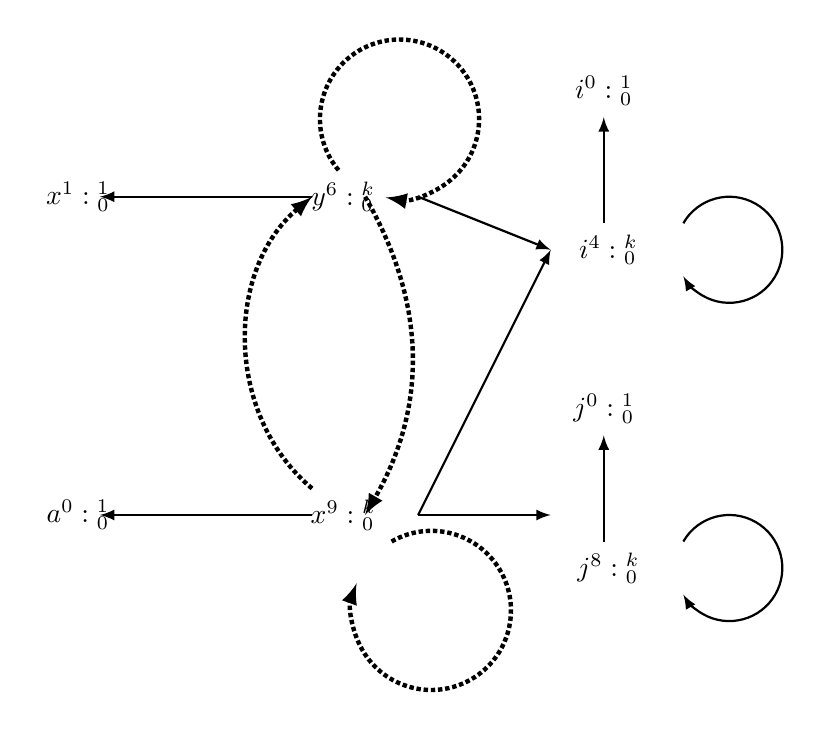
\begin{tikzpicture}[scale=\textwidth/18cm,samples=200]
% Variables Initialization
\draw[] (-5, 1) circle (0pt) node{{ $a^0: {}^1_{0}$}};
\draw[] (-5, 7) circle (0pt) node{{ $x^1: {}^{1}_{0}$}};
% Variables Inside the Loop
   \draw[] (0, 7) circle (0pt) node{{ $y^6: {}^{k}_{0}$}};
   \draw[] (0, 1) circle (0pt) node{{ $x^9: {}^{k}_{0}$}};
   % Counter Variables
   \draw[] (5, 9) circle (0pt) node {{$i^0: {}^{1}_{0}$}};
   \draw[] (5, 6) circle (0pt) node {{ $i^4: {}^{k}_{0}$}};
   \draw[] (5, 3) circle (0pt) node {{$j^0: {}^{1}_{0}$}};
   \draw[] (5, 0) circle (0pt) node {{ $j^8: {}^{k}_{0}$}};
   %
   % Value Dependency Edges:
   \draw[ ultra thick, -latex, densely dotted,] (0, 7.5) arc (220:-100:1.5);
   \draw[ thick, -latex] (5, 6.5)  -- (5, 8.5) ;
   \draw[ thick, -latex] (5, 0.5)  -- (5, 2.5) ;
   \draw[ ultra thick, -latex, densely dotted,] (1., 0.5) arc (120:-200:1.5);
   % Value Dependency Edges on Initial Values:
   \draw[ thick, -latex,] (-0.5, 1)  -- (-4.5, 1) ;
   \draw[ thick, -latex,] (-0.5, 7)  -- (-4.5, 7) ;
   %
   \draw[ ultra thick, -latex, densely dotted,] (-0.5, 1.5)  to  [out=-220,in=220]  (-0.5, 7);
   \draw[ ultra thick, -latex, densely dotted,]  (0.5, 7) to  [out=-60,in=60] (0.5, 1) ;
   % Control Dependency
  %  \draw[ thick,-latex] (1.5, 7)  -- (4, 9) ;
  %  \draw[ thick,-latex] (1.5, 4)  -- (4, 9) ;
  \draw[ thick, -latex, ] (6.5, 6.5) arc (150:-150:1);
  \draw[ thick, -latex, ] (6.5, 0.5) arc (150:-150:1);
  \draw[ thick,-latex] (1.5, 7)  -- (4, 6) ;
   \draw[ thick,-latex] (1.5, 1)  -- (4, 6) ;
   \draw[ thick,-latex] (1.5, 1)  -- (4, 1) ;
   \end{tikzpicture}
   \caption{}
      \end{centering}
      \end{subfigure}
    }
    % \end{wrapfigure}
    % \end{equation*}
    \vspace{-0.4cm}
     \caption{(a) Nested While Loop Example, (b) Execution-Based Dependency Graph, (c) The Static Program-Based Dependency graph.}
    \label{fig:alg_adaptsearch_nestedwhile}
    \vspace{-0.5cm}
    \end{figure}
    %
%     When we searched for a walk: $y^6 \to y^6$,
%   if we update the $\kw{flowcapacity}[y^6]$ as $k$ after visiting $y^6$ the second time 
%   on this walk,
%   % the walk $y^6 \to y^6$,
%   and continuously visit $x^9$,
%   then the $\kw{flowcapacity[k]}$ is 
%   updated as $\min(k, k^2)$.
%   So
%   %  which 
%   % restricting 
%   the visiting times of $x^9$ is restricted by $k$ on the walk $y^6 \to y^6 \to x^9$.
%   This restriction excludes the finite walk $y^6 \to y^6 \to x^9 \to x^9$ where $y^6$ and $x^9$ visited by $k^2$ times
%   in the computation. 
%   However, the finite walk $y^6 \to y^6 \to x^9 \to x^9$ where $y^6$ is visited $k$ times and $x^9$ $k^2$ times is 
%   a qualified walk, and exactly the longest walk we aim to find. So, by Non-updating the $\kw{flowcapacity}$ after 
%   visiting $y$ again, we guarantee that the visiting times og vertices on every searched walk will not be restricted by weights not on this walk,
%   i.e., the soundness.
%  \\
% In the last line of this dfs algorithm, line: 16, it returns the adaptivity heading out from its input vertex.
% \\
% By applying this deep first search strategy on every vertex on this SCC, 
% we compute the adaptivity of this SCC by taking the maximum 
% % adaptivity reaching every vertex on this SCC.
% value over every vertex.
% %
% The soundness is formally guaranteed in Lemma~\ref{lem:sound_adaptalg_scc} in Appendix~\ref{apdx:adaptalg_soundness}.
            % \begin{algorithm}
        % \caption{
        % {Refined Adaptivity on $\kw{SCC}$}
        % \label{alg:dfscycle_alg}
        % }
        % \begin{algorithmic}
        % \REQUIRE Weighted Directed Graph $G = (\vertxs, \edges, \weights, \qflag)$ with a start vertex $s$ and destination vertex $t$ .
        % \STATE  {\bf {$\kw{dfs_{refine}(G, c, visited)}$}:}  
        % \STATE {\bf init} 
        % \\
        % current node: $c$, 
        % % \\
        % % visited: List of length $|\vertxs|$, initialize with $\efalse$.
        % \\
        % results: $r$ : INT List of length $|\vertxs|$, initialize with $\qflag(v)$ for every vertex.
        % \\
        % $\kw{flowcapacity}$: INT List of length $|\vertxs|$, initialize MAXINT. 
        % \#\{For every vertex, recording the minimum weight when the walk reaching 
        % that vertex, inside a cycle\}
        % \\
        % querynum: INT List of length $|\vertxs|$, initialize with $\qflag(v)$ for every vertex. 
        % \#\{For every vertex, recording the query numbers when the walk reaching 
        % that vertex, inside a cycle\}
        % \\
        % % \STATE {\bf if} $c = s$:
        % % \STATE \qquad update the length of the longest path reaching this vertex
        % % $r[s] =  r[s] + $$\kw{flowcapacity}$[s] * querynum[s].
        % % \RETURN  \qquad $r[s]$.      
        % \STATE {\bf for}  all vertex $v$ having directed edge from $c$:
        % \STATE \qquad \qquad $\kw{flowcapacity}$[v] = min($\weights(v)$, $\kw{flowcapacity}$[c]);
        % \STATE \qquad \qquad querynum[v] = querynum[c] + $\qflag(v)$;
        % \STATE \qquad \qquad \#\{do not update the length of the longest walk reaching $v$ until the cycle is finished\}
        % \STATE \qquad \qquad $r[v] =  r[c] $;
        % \STATE \qquad {\bf if}  $v$ is unvisited:
        % \STATE \qquad \qquad \#\{mark $v$ as visited\} $\kw{visited}[v] = 1$;
        % \STATE \qquad \qquad $\kw{dfs_{refine}(G, v, visited)}$;
        % \STATE \qquad {\bf else}: \#\{There is a cycle finished\}
        % \STATE \qquad \qquad \#\{update the length of the longest path reaching this vertex\}
        % \STATE \qquad \qquad 
        %  $r[v] =  \max(r[v], r[c] + $$\kw{flowcapacity}$[v] * querynum[v]);
        %  \STATE \qquad \qquad \#\{Recover the $\kw{flowcapacity}$ and querynumber to previous state, for different loops\}
        %  \STATE \qquad \qquad $\kw{flowcapacity}$[v] = $\kw{flowcapacity}$[c];
        %  \STATE \qquad \qquad querynum[v] = querynum[c];
        % \RETURN  $r[c]$
        % \end{algorithmic}
        % \end{algorithm}
        % %
        \begin{algorithm}
          \caption{
          {Over-Approximated Adaptivity on SCC}
          \label{alg:overadp_alg}
          }
          \begin{algorithmic}[1]
          \REQUIRE $G = (\vertxs, \edges, \weights, \qflag)$ \#\{An Strong Connected Symbolic Weighted Directed Graph\}
          % with a start vertex $s$ and destination vertex $t$ .
          \STATE {\bf {$\kw{\pathsearch_{scc-naive}(G)}$}:}  
          \STATE {\bf init} 
          \\
          $\kw{r_{scc}}$: the Adaptivity of this SCC
          % \STATE  {\bf def} {$\kw{dfs_{naive}(G, c,visited)}$}: 
          % % \STATE {\bf init} 
          % % \\
          % % current node: $c$, 
          % % \\
          % % visited: List of length $|\vertxs|$, initialize with $\efalse$.
          % % \\
          % % \STATE {\bf if} $c = s$:
          % % \RETURN \qquad  $\weights(s)*\flag(s) $.
          % \STATE \qquad $r[c] = \weights(c)*\qflag(c) $
          % \STATE \qquad {\bf for}  all vertex $v$ having directed edge from $c$:
          % \STATE \qquad \qquad {\bf if}  $v$ is unvisited:
          % \STATE \qquad \qquad \qquad  \#\{mark $v$ as visited\} $\kw{visited}[v] = 1$;
          % \STATE \qquad \qquad \qquad $r[c] += \kw{dfs_{naive}(G, v, visited)}$;
          % \STATE \qquad {\bf else}: \#\{There is a cycle finished\}
          % \RETURN \qquad \qquad $\weights(v)*\flag(v) $.
          \STATE  {\bf for} every vertex $v$ in $\vertxs$:
          % \STATE  \qquad initialize \kw{visited} with $\efalse$.
          \STATE  \qquad $r_{scc} += \weights(v)*\qflag(v)$  
          \RETURN $r[c]$
          \end{algorithmic}
          \end{algorithm}
          %
\begin{thm}[Soundness of $\pathsearch$]
    \label{thm:sound_adaptalg}
    For every program $c$, given its \emph{Program-Based Dependency Graph} $\progG$,
     $$\pathsearch(\progG) \geq \progA(\progG).$$
\end{thm}